% Saberes básicos (LOMLOE) asociados a esta unidad
%
% D. La interacción
%   - Las fuerzas como agentes de cambio: relación de los efectos de las fuerzas, tanto en el
%     estado de movimiento o de reposo de un cuerpo como produciendo deformaciones en los
%     sistemas sobre los que actúan: se trata explícitamente en "Las fuerzas y el movimiento. Leyes
%     de Newton" y en "Fuerzas y deformación" (cuerpos rígidos, elásticos y plásticos, ley de Hooke).
%   - Aplicación de las leyes de Newton: observación de situaciones cotidianas o de laboratorio
%     que permiten entender cómo se comportan los sistemas materiales ante la acción de las
%     fuerzas y predecir los efectos de estas en situaciones cotidianas y de seguridad vial:
%     las tres leyes de Newton se presentan con ejemplos cotidianos (patinadores, coches,
%     cinturón de seguridad) y se añade un apartado específico de fricción y seguridad vial
%     (distancia de frenado, cinturón de seguridad, airbag, distancia de seguridad).
%   - Fenómenos gravitatorios: el peso como fuerza de atracción gravitatoria se relaciona con
%     la masa y con las leyes de Newton (segunda ley aplicada a la caída libre).
%
% A. Las destrezas científicas básicas
%   - Unidades del Sistema Internacional: uso sistemático de \unit{} y \qty{} (N, N/m, m/s^2).
%
% (Traducción al español de Unit_8_Forces.tex. La cinemática está en la Unidad 7, Movimiento.)

\spacing{1.3}
\raggedbottom % pages with large figures end where the text ends (no stretched gaps between boxes)

\section{Introducción}

En la unidad anterior aprendimos a describir el movimiento. En esta unidad estudiaremos su causa: las \textbf{fuerzas}. Veremos qué es una fuerza, cómo explican las \textbf{leyes de Newton} la manera en que las fuerzas cambian el movimiento de los cuerpos, en qué se diferencian el \textbf{peso} y la \textbf{masa}, y cómo las fuerzas también pueden \textbf{deformar} los objetos.

\section{Las fuerzas y el movimiento. Leyes de Newton}

\subsection{¿Qué es una fuerza?}

\begin{definition}[Fuerza]
    Es toda acción capaz de \textbf{cambiar el estado de movimiento} de un cuerpo (hacer que empiece a moverse, que se pare, que vaya más deprisa o más despacio, o que cambie de dirección) o de \textbf{deformarlo}. Se representa con la letra \(F\) y, en el SI, se mide en \textbf{newtons} (\unit{\newton}).
\end{definition}

\begin{impt}
    \negsubro{Las fuerzas son la causa de los cambios en el movimiento}:
    \begin{itemize}
        \item Las fuerzas son las que hacen que los objetos \textbf{empiecen a moverse}, y las que hacen que \textbf{aceleren, frenen, se paren o giren}.
        \item Si sobre un objeto \textbf{no actúa ninguna fuerza} (o todas las fuerzas se anulan entre sí), el objeto \textbf{no se mueve} si estaba en reposo, o sigue moviéndose \textbf{con velocidad constante} en línea recta. En los dos casos su velocidad no cambia, así que su \textbf{aceleración es cero} (\(a = 0\)).
    \end{itemize}
\end{impt}

\begin{definition}[Newton, N]
    Es la unidad de fuerza del SI. Una fuerza de \qty{1}{\newton} que actúa sobre un objeto de \qty{1}{\kg} le produce una aceleración de \qty{1}{\mpss}, en la misma dirección y sentido que la fuerza.
\end{definition}

El científico inglés Isaac Newton (1642--1727) descubrió tres leyes que explican cómo cambian las fuerzas el movimiento de los objetos.

\begin{figure}[H]
    \centering
    % [FIGURA ORIGINAL] \includegraphics[width=\textwidth]{Unit_8/newton_laws}
    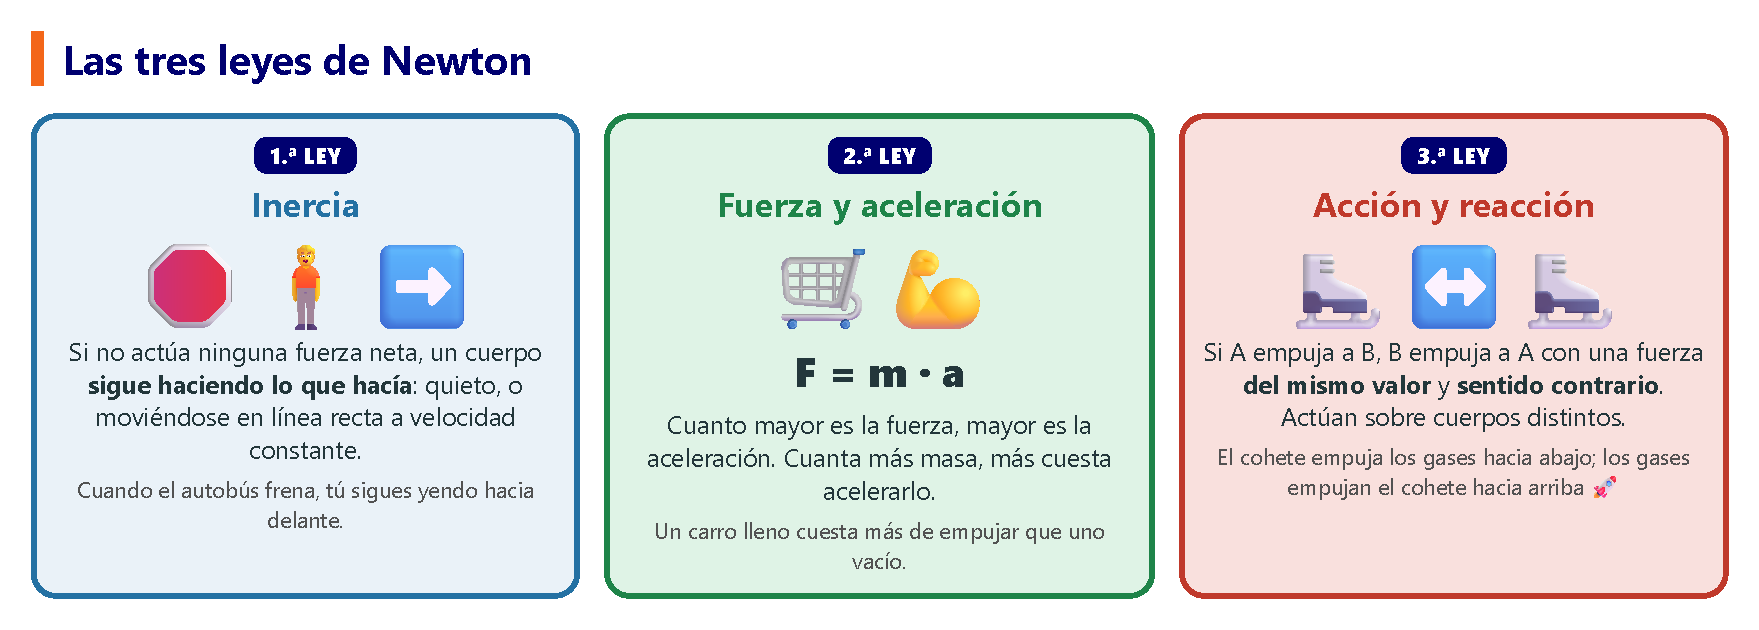
\includegraphics[width=\textwidth]{FigurasSVG/Unit_8_Forces/pdf/newton_laws_es.pdf}
    \caption{Las tres leyes de Newton del movimiento.}
    \label{fig:u8_newton_laws}
\end{figure}

\subsection{Primera ley de Newton: ley de la inercia}

\begin{definition}[Primera ley de Newton]
    Si sobre un cuerpo no actúa ninguna fuerza (o las fuerzas que actúan sobre él se anulan), el cuerpo sigue \textbf{en reposo} si estaba en reposo, o sigue moviéndose en \textbf{línea recta con velocidad constante} (MRU) si estaba en movimiento.
\end{definition}

Los cuerpos «prefieren» seguir haciendo lo que estaban haciendo: esta tendencia a resistirse a los cambios en su movimiento se llama \negsubro{inercia}. Cuanta más masa tiene un cuerpo, más inercia tiene: cuesta más empezar a empujar un coche que una bicicleta, y también cuesta más pararlo.

\begin{example}
    \begin{itemize}
        \item Cuando un autobús frena de golpe, los pasajeros se van \textbf{hacia delante}: su cuerpo tiende a seguir moviéndose a la velocidad que llevaba el autobús.
        \item Cuando un autobús arranca de golpe, los pasajeros se van \textbf{hacia atrás}: su cuerpo tiende a seguir en reposo.
        \item Un disco de hockey se desliza un largo trecho sobre el hielo, porque casi no hay rozamiento que lo frene.
    \end{itemize}
\end{example}

\subsection{Segunda ley de Newton: ley fundamental de la dinámica}

\begin{definition}[Segunda ley de Newton]
    Cuando una fuerza (neta) actúa sobre un cuerpo, le produce una \textbf{aceleración} en la misma dirección y sentido que la fuerza. La fuerza es igual a la masa del cuerpo multiplicada por su aceleración:
    \begin{equation*}
        F = m \cdot a
    \end{equation*}
    donde \(F\) es la fuerza (\unit{\newton}), \(m\) la masa (\unit{\kg}) y \(a\) la aceleración (\unit{\mpss}).
\end{definition}

\begin{impt}
    \begin{itemize}
        \item Cuanto \textbf{mayor es la fuerza}, \textbf{mayor es la aceleración}: si empujamos más fuerte, el objeto acelera más.
        \item Cuanto \textbf{mayor es la masa}, \textbf{menor es la aceleración}: con el mismo empujón, un carro vacío acelera más que uno lleno.
        \item Si la fuerza es cero, la aceleración es cero: es otra vez la primera ley.
    \end{itemize}
\end{impt}

En los ejercicios nos pueden pedir la fuerza, la masa o la aceleración. Para calcular \(m\) o \(a\), primero las \textbf{despejamos}, como hicimos con la densidad y la velocidad:

\begin{figure}[H]
    \centering
    % [FIGURA ORIGINAL] \includegraphics[width=\textwidth]{Unit_8/newton2_isolate}
    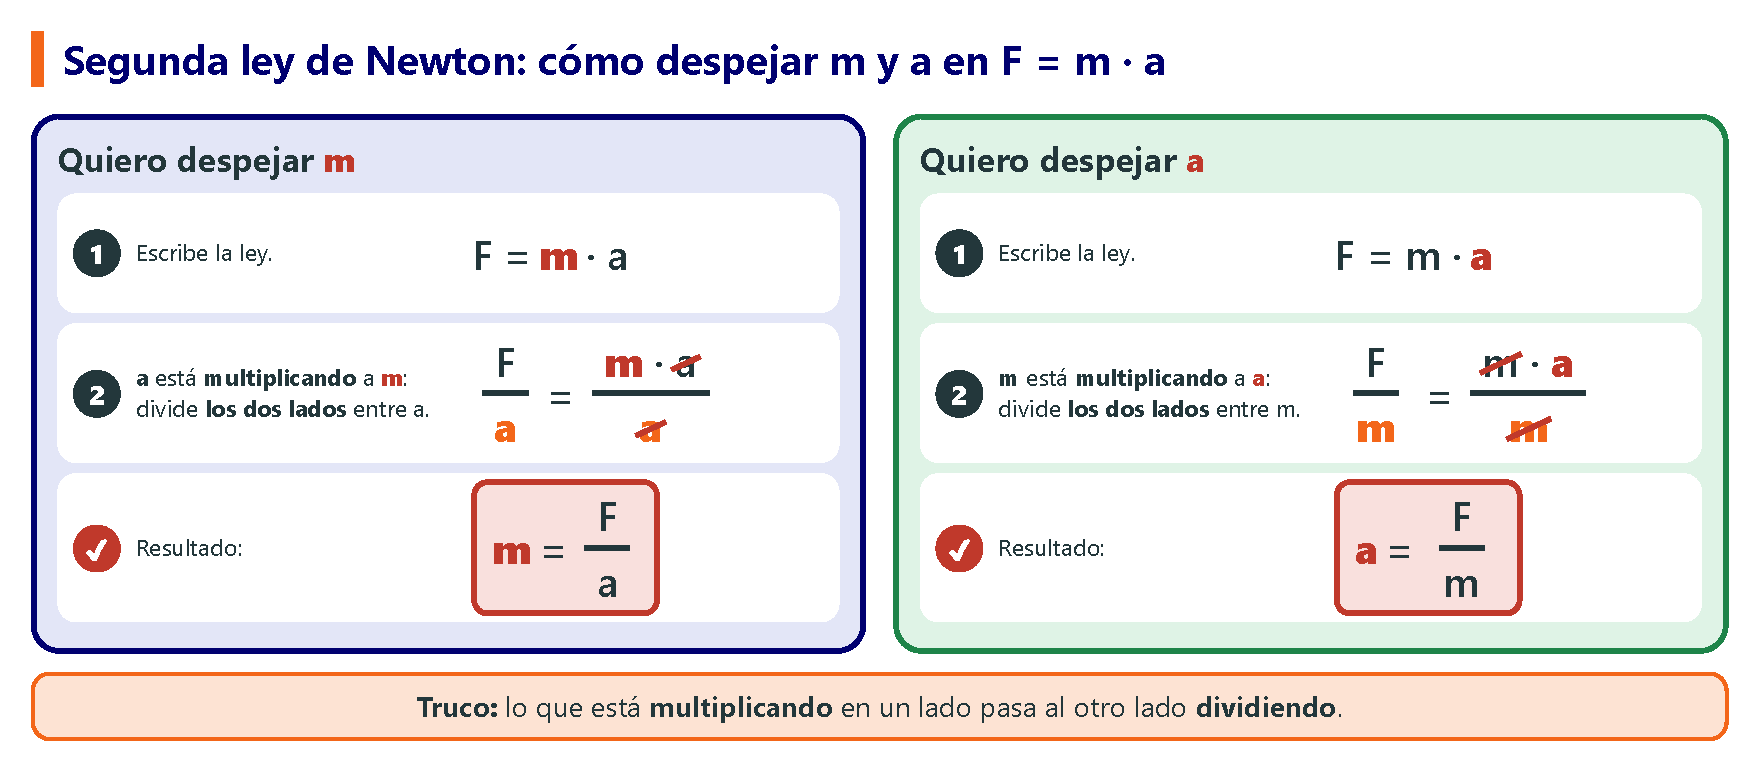
\includegraphics[width=\textwidth]{FigurasSVG/Unit_8_Forces/pdf/newton2_isolate_es.pdf}
    \caption{Cómo despejar la masa y la aceleración en \(F = m \cdot a\), paso a paso.}
    \label{fig:u8_newton2_isolate}
\end{figure}

\begin{itemize}
    \item \textbf{Masa}: \(a\) está multiplicando a \(m\), así que dividimos los dos lados entre \(a\):
    \(\;\dfrac{F}{a} = \dfrac{m \cdot \cancelred{a}}{\cancelred{a}} \;\Rightarrow\; \textcolor{red}{m = \dfrac{F}{a}}\)
    \item \textbf{Aceleración}: \(m\) está multiplicando a \(a\), así que dividimos los dos lados entre \(m\):
    \(\;\dfrac{F}{m} = \dfrac{\cancelred{m} \cdot a}{\cancelred{m}} \;\Rightarrow\; \textcolor{red}{a = \dfrac{F}{m}}\)
\end{itemize}

\begin{impt}
    Las tres formas de la segunda ley de Newton:
    \begin{equation*}
        F = m \cdot a \qquad\qquad m = \dfrac{F}{a} \qquad\qquad a = \dfrac{F}{m}
    \end{equation*}
\end{impt}

\begin{example}
    \textbf{Cálculo de una fuerza. ¿Qué fuerza hace falta para darle a un carro de \qty{50}{\kg} una aceleración de \qty{2}{\mpss}?}
    \begin{enumerate}[label=\numberballmDarkTeal]
        \item Datos: \(m = \qty{50}{\kg}\), \(a = \qty{2}{\mpss}\). Incógnita: \(\underline{F}\).
        \item Fórmula: \(F = m \cdot a\) (no hace falta despejar).
        \item \(F = \qty{50}{\kg} \cdot \qty{2}{\mpss} = \textcolor{red}{\qty{100}{\newton}}\).
    \end{enumerate}
\end{example}

\begin{example}
    \textbf{Cálculo de una masa. Una fuerza de \qty{300}{\newton} le da a una moto una aceleración de \qty{1.5}{\mpss}. ¿Cuál es la masa de la moto?}
    \begin{enumerate}[label=\numberballmDarkTeal]
        \item Datos: \(F = \qty{300}{\newton}\), \(a = \qty{1.5}{\mpss}\). Incógnita: \(\underline{m}\).
        \item Fórmula: \(F = m \cdot a\). \(a\) está multiplicando a \(m\), así que pasa al otro lado dividiendo: \(m = \dfrac{F}{a}\).
        \item \(m = \dfrac{\qty{300}{\newton}}{\qty{1.5}{\mpss}} = \textcolor{red}{\qty{200}{\kg}}\).
    \end{enumerate}
\end{example}

\begin{example}
    \textbf{Cálculo de una aceleración. Una fuerza de \qty{60}{\newton} empuja una caja de \qty{12}{\kg}. ¿Qué aceleración adquiere?}
    \begin{enumerate}[label=\numberballmDarkTeal]
        \item Datos: \(F = \qty{60}{\newton}\), \(m = \qty{12}{\kg}\). Incógnita: \(\underline{a}\).
        \item Fórmula: \(F = m \cdot a\). \(m\) está multiplicando a \(a\), así que pasa al otro lado dividiendo: \(a = \dfrac{F}{m}\).
        \item \(a = \dfrac{\qty{60}{\newton}}{\qty{12}{\kg}} = \textcolor{red}{\qty{5}{\mpss}}\).
    \end{enumerate}
\end{example}

\begin{exercise}
    \textbf{Calcula la fuerza} en cada caso:
    \begin{enumerate}[label=\letraminuscula]
        \item Un coche de \qty{1200}{\kg} acelera a \qty{3}{\mpss}.
        \item Se da una patada a un balón de fútbol de \qty{0.45}{\kg} y adquiere una aceleración de \qty{200}{\mpss}.
        \item Una ciclista de \qty{70}{\kg} (con su bici) acelera a \qty{0.5}{\mpss}.
    \end{enumerate}
    \begin{solu}
        \begin{enumerate}[label=\alph*)]
            \item \(F = m \cdot a = \qty{1200}{\kg} \cdot \qty{3}{\mpss} = \qty{3600}{\newton}\).
            \item \(F = \qty{0.45}{\kg} \cdot \qty{200}{\mpss} = \qty{90}{\newton}\).
            \item \(F = \qty{70}{\kg} \cdot \qty{0.5}{\mpss} = \qty{35}{\newton}\).
        \end{enumerate}
    \end{solu}
\end{exercise}

\begin{exercise}
    \textbf{Calcula la masa} en cada caso:
    \begin{enumerate}[label=\letraminuscula]
        \item Una fuerza de \qty{20}{\newton} produce una aceleración de \qty{4}{\mpss}.
        \item Una fuerza de \qty{4500}{\newton} le da a una furgoneta una aceleración de \qty{1.5}{\mpss}.
        \item Una fuerza de \qty{9}{\newton} le da a un monopatín una aceleración de \qty{3}{\mpss}.
    \end{enumerate}
    \begin{solu}
        \begin{enumerate}[label=\alph*)]
            \item \(m = \dfrac{F}{a} = \dfrac{\qty{20}{\newton}}{\qty{4}{\mpss}} = \qty{5}{\kg}\).
            \item \(m = \dfrac{\qty{4500}{\newton}}{\qty{1.5}{\mpss}} = \qty{3000}{\kg}\).
            \item \(m = \dfrac{\qty{9}{\newton}}{\qty{3}{\mpss}} = \qty{3}{\kg}\).
        \end{enumerate}
    \end{solu}
\end{exercise}

\begin{exercise}
    \textbf{Calcula la aceleración} en cada caso:
    \begin{enumerate}[label=\letraminuscula]
        \item Una fuerza de \qty{40}{\newton} actúa sobre un trineo de \qty{8}{\kg}.
        \item Una fuerza de \qty{2000}{\newton} actúa sobre una barca de \qty{500}{\kg}.
        \item Una fuerza de \qty{15}{\newton} actúa sobre una pelota de \qty{0.5}{\kg}.
    \end{enumerate}
    \begin{solu}
        \begin{enumerate}[label=\alph*)]
            \item \(a = \dfrac{F}{m} = \dfrac{\qty{40}{\newton}}{\qty{8}{\kg}} = \qty{5}{\mpss}\).
            \item \(a = \dfrac{\qty{2000}{\newton}}{\qty{500}{\kg}} = \qty{4}{\mpss}\).
            \item \(a = \dfrac{\qty{15}{\newton}}{\qty{0.5}{\kg}} = \qty{30}{\mpss}\).
        \end{enumerate}
    \end{solu}
\end{exercise}

\begin{exercise}
    Calcula la aceleración que produce una fuerza de \qty{5}{\newton} sobre un objeto de \qty{2}{\kg} de masa.
    \begin{enumerate}[label=\letraminuscula]
        \item ¿Qué fuerza tendríamos que aplicar a un objeto de \qty{10}{\kg} para producirle la misma aceleración?
    \end{enumerate}
    \begin{solu}
        \(a = \dfrac{F}{m} = \dfrac{\qty{5}{\newton}}{\qty{2}{\kg}} = \qty{2.5}{\mpss}\). \\
        Para la misma aceleración con \qty{10}{\kg}: \(F = m \cdot a = \qty{10}{\kg} \cdot \qty{2.5}{\mpss} = \qty{25}{\newton}\).
    \end{solu}
\end{exercise}

\begin{exercise}
    Un coche de \qty{1000}{\kg} de masa tiene una fuerza del motor de \qty{2000}{\newton} y sobre él actúa en contra una fuerza de rozamiento de \qty{1500}{\newton}. Calcula su aceleración.
    \begin{solu}
        Fuerza neta \(= \qty{2000}{\newton} - \qty{1500}{\newton} = \qty{500}{\newton}\) (en el sentido del movimiento). \\
        \(a = \dfrac{F}{m} = \dfrac{\qty{500}{\newton}}{\qty{1000}{\kg}} = \qty{0.5}{\mpss}\).
    \end{solu}
\end{exercise}

\begin{exercise}
    Una fuerza neta de \qty{12}{\newton} que actúa sobre un objeto le produce una aceleración de \qty{3}{\mpss}.
    \begin{enumerate}[label=\letraminuscula]
        \item Calcula la masa del objeto.
        \item Si empujáramos el mismo objeto con una fuerza neta de \qty{24}{\newton}, ¿qué aceleración tendría?
    \end{enumerate}
    \begin{solu}
        \begin{enumerate}[label=\alph*)]
            \item \(m = \dfrac{F}{a} = \dfrac{\qty{12}{\newton}}{\qty{3}{\mpss}} = \qty{4}{\kg}\).
            \item \(a = \dfrac{F}{m} = \dfrac{\qty{24}{\newton}}{\qty{4}{\kg}} = \qty{6}{\mpss}\).
        \end{enumerate}
    \end{solu}
\end{exercise}


\subsection{Tercera ley de Newton: acción y reacción}

\begin{definition}[Tercera ley de Newton]
    Cuando un cuerpo ejerce una fuerza sobre otro cuerpo (\textbf{acción}), el segundo cuerpo ejerce sobre el primero una fuerza del \textbf{mismo valor} pero de \textbf{sentido contrario} (\textbf{reacción}).
\end{definition}

\begin{impt}
    Las fuerzas siempre aparecen \textbf{por parejas}. La acción y la reacción actúan sobre \textbf{cuerpos distintos}, así que \textbf{no se anulan} entre sí.
\end{impt}

\begin{example}
    Una patinadora empuja a otro patinador. Los dos se mueven hacia atrás: el empujón es la \textbf{acción}, y la fuerza que echa hacia atrás a la primera patinadora es la \textbf{reacción}. Las dos fuerzas tienen el mismo valor pero sentidos contrarios, y actúan sobre personas distintas, así que no se anulan.
\end{example}

\begin{example}
    \begin{itemize}
        \item \textbf{Al andar}: nuestro pie empuja el suelo hacia atrás (acción) y el suelo nos empuja hacia delante (reacción).
        \item \textbf{Al nadar}: empujamos el agua hacia atrás con las manos y el agua nos empuja hacia delante.
        \item \textbf{Un cohete}: empuja los gases hacia abajo y los gases empujan el cohete hacia arriba.
    \end{itemize}
\end{example}

\begin{impt}
    \negsubro{Relación entre fuerzas y movimiento}:
    \begin{itemize}
        \item No actúa ninguna fuerza neta \(\to\) el objeto sigue \textbf{en reposo} o mantiene su \textbf{MRU} (\(a = 0\)).
        \item Una fuerza neta cambia el \textbf{valor} de la velocidad de manera uniforme \(\to\) \textbf{MRUA}.
        \item Una fuerza neta cambia solo la \textbf{dirección} del movimiento (no la rapidez) \(\to\) \textbf{movimiento circular}.
    \end{itemize}
\end{impt}

\subsection{Peso y masa}

\begin{impt}
    \negsubro{El peso es una fuerza}: es la fuerza con la que un astro (como la Tierra) atrae a una masa hacia su centro. No hay que confundirlo con la masa:
    \begin{itemize}
        \item \textbf{Masa} (\(m\)): la cantidad de materia de un cuerpo. Se mide en \unit{\kg} y \textbf{no} cambia de un lugar a otro.
        \item \textbf{Peso} (\(P\)): la fuerza de la gravedad que actúa sobre esa masa. Se mide en \unit{\newton} y \textbf{sí} cambia: es distinto en la Luna que en la Tierra.
    \end{itemize}
\end{impt}

\begin{definition}[Peso]
    El peso de un objeto es igual a su masa por la aceleración de la gravedad (aplicando la segunda ley de Newton):
    \begin{equation*}
        P = m \cdot g
    \end{equation*}
    En la Tierra, \(g \approx \qty{9.8}{\mpss}\) (a menudo se redondea a \qty{10}{\mpss}).
\end{definition}

\begin{figure}[H]
    \centering
    % [FIGURA ORIGINAL] \includegraphics[width=\textwidth]{Unit_8/weight_planets}
    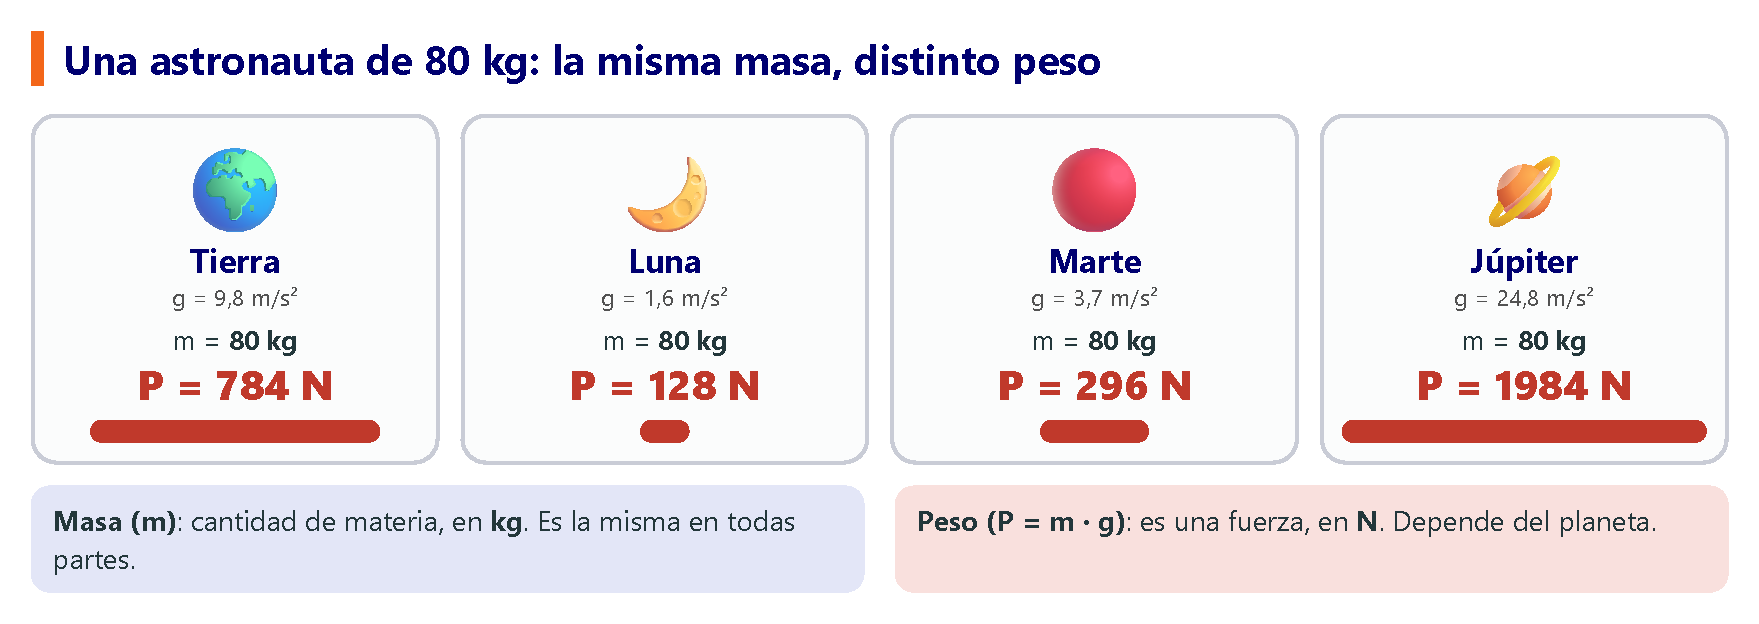
\includegraphics[width=\textwidth]{FigurasSVG/Unit_8_Forces/pdf/weight_planets_es.pdf}
    \caption{La masa de la astronauta es la misma en todas partes; el peso depende de la gravedad de cada lugar.}
    \label{fig:u8_weight_planets}
\end{figure}

\begin{example}
    \textbf{Calcula el peso de un alumno de \qty{60}{\kg} en la Tierra (\(g=\qty{9.8}{\mpss}\)) y en la Luna (\(g_{\text{Luna}} \approx \qty{1.6}{\mpss}\)).}
    \begin{equation*}
        P_{\text{Tierra}} = \qty{60}{\kg} \cdot \qty{9.8}{\mpss} = \qty{588}{\newton}
        \qquad
        P_{\text{Luna}} = \qty{60}{\kg} \cdot \qty{1.6}{\mpss} = \qty{96}{\newton}
    \end{equation*}
    La \textbf{masa} del alumno (\qty{60}{\kg}) es la misma en los dos sitios; solo cambia el \textbf{peso}, porque \(g\) es distinta.
\end{example}

\begin{exercise}
    Una astronauta tiene una masa de \qty{80}{\kg}.
    \begin{enumerate}[label=\letraminuscula]
        \item Calcula su peso en la Tierra (\(g=\qty{9.8}{\mpss}\)).
        \item Calcula su peso en Marte, donde \(g_{\text{Marte}} \approx \qty{3.7}{\mpss}\).
        \item ¿Cambia su masa entre la Tierra y Marte?
    \end{enumerate}
    \begin{solu}
        \begin{enumerate}[label=\alph*)]
            \item \(P_{\text{Tierra}} = \qty{80}{\kg} \cdot \qty{9.8}{\mpss} = \qty{784}{\newton}\).
            \item \(P_{\text{Marte}} = \qty{80}{\kg} \cdot \qty{3.7}{\mpss} = \qty{296}{\newton}\).
            \item No: su \textbf{masa} sigue siendo \qty{80}{\kg} en los dos planetas; solo cambia su \textbf{peso}, porque depende de \(g\).
        \end{enumerate}
    \end{solu}
\end{exercise}

\begin{exercise}
    Una caja pesa \qty{500}{\newton} en la Tierra (\(g=\qty{10}{\mpss}\)).
    \begin{enumerate}[label=\letraminuscula]
        \item Calcula su masa.
        \item Calcula su peso en la Luna (\(g_{\text{Luna}} \approx \qty{1.6}{\mpss}\)).
    \end{enumerate}
    \begin{solu}
        \begin{enumerate}[label=\alph*)]
            \item \(m = \dfrac{P}{g} = \dfrac{\qty{500}{\newton}}{\qty{10}{\mpss}} = \qty{50}{\kg}\).
            \item \(P_{\text{Luna}} = m \cdot g_{\text{Luna}} = \qty{50}{\kg} \cdot \qty{1.6}{\mpss} = \qty{80}{\newton}\).
        \end{enumerate}
    \end{solu}
\end{exercise}

\begin{exercise}
    El objeto \(X\) tiene una masa de \qty{10}{\kg} y el objeto \(Y\), una masa de \qty{20}{\kg}. Los dos se llevan a Júpiter, donde \(g_{\text{Júpiter}} \approx \qty{24.8}{\mpss}\).
    \begin{enumerate}[label=\letraminuscula]
        \item Calcula el peso de cada objeto en Júpiter.
        \item ¿Qué objeto pesa más? ¿Seguiría siendo así si los comparáramos en la Tierra?
    \end{enumerate}
    \begin{solu}
        \begin{enumerate}[label=\alph*)]
            \item \(P_X = \qty{10}{\kg} \cdot \qty{24.8}{\mpss} = \qty{248}{\newton}\). \\
            \(P_Y = \qty{20}{\kg} \cdot \qty{24.8}{\mpss} = \qty{496}{\newton}\).
            \item \(Y\) pesa más, porque tiene más masa. Como \(P = m \cdot g\) y \(g\) es la misma para los dos objetos en un mismo lugar, el objeto con más masa siempre pesa más allí; así que sí, \(Y\) también pesaría más que \(X\) en la Tierra.
        \end{enumerate}
    \end{solu}
\end{exercise}

%\subsection{Friction force}
%
%\begin{definition}[Friction force]
%    A force that opposes the relative motion (or attempted motion) between two surfaces in contact. It always acts \textbf{opposite} to the direction of motion.
%\end{definition}
%
%\begin{itemize}
%    \item Friction depends on the \textbf{nature of the surfaces} in contact: rough surfaces produce more friction than smooth, polished ones.
%    \item Friction \textbf{opposes motion}, so it is often an unwanted effect (it wastes energy and wears out machine parts, so we reduce it with lubricants, ball bearings, or by polishing surfaces).
%    \item Friction is also \textbf{necessary}: without it, we could not walk, cars could not grip the road, and objects would slide off any tilted surface.
%\end{itemize}
%
%\begin{figure}[H]
%    \centering
%    \includegraphics[width=0.95\textwidth]{Unit_8/free_body}
%    \caption{Forces acting on a box pushed along the floor.}
%    \label{fig:u8_free_body}
%\end{figure}
%
%\begin{example}
%    A box is pushed with a force of \qty{50}{\newton} along the floor, while a frictional force of \qty{50}{\newton} opposes it. Since the net force is zero, the box moves at \textbf{constant speed} (or stays at rest), by Newton's first law.
%\end{example}
%
%\begin{exercise}
%    A wooden crate is pushed with a force of \qty{80}{\newton} across a rough floor, while the floor exerts a frictional force of \qty{80}{\newton} against it, in the opposite direction.
%    \begin{enumerate}[label=\letraminuscula]
%        \item Calculate the net force acting on the crate.
%        \item According to Newton's first law, what happens to the crate's motion?
%    \end{enumerate}
%    \begin{solu}
%        \begin{enumerate}[label=\alph*)]
%            \item Net force \(= \qty{80}{\newton} - \qty{80}{\newton} = \qty{0}{\newton}\).
%            \item Since the net force is zero, the crate's state of motion does not change: if it was at rest, it stays at rest; if it was already moving, it keeps moving with URM (constant speed).
%        \end{enumerate}
%    \end{solu}
%\end{exercise}
%
%\begin{exercise}
%    A sled of mass \qty{20}{\kg} is pulled with a force of \qty{100}{\newton}, while friction opposes its motion with a force of \qty{40}{\newton}.
%    \begin{enumerate}[label=\letraminuscula]
%        \item Calculate the net force.
%        \item Calculate the sled's acceleration.
%    \end{enumerate}
%    \begin{solu}
%        \begin{enumerate}[label=\alph*)]
%            \item Net force \(= \qty{100}{\newton} - \qty{40}{\newton} = \qty{60}{\newton}\).
%            \item \(a = \dfrac{F}{m} = \dfrac{\qty{60}{\newton}}{\qty{20}{\kg}} = \qty{3}{\mpss}\).
%        \end{enumerate}
%    \end{solu}
%\end{exercise}
%
%\begin{exercise}
%    Explain why a car's tyres need enough friction (grip) with the road to accelerate, brake and turn corners safely, and why an icy road makes all of this more difficult.
%    \begin{solu}
%        The engine's driving force, the braking force, and the force needed to change direction in a corner are all transmitted to the road through friction between the tyres and the road surface. On an icy road, friction is much smaller, so the maximum forces the tyres can exert are also much smaller: the car needs a longer distance to accelerate or brake, and can lose grip (skid) more easily when turning.
%    \end{solu}
%\end{exercise}

\subsection{Las leyes de Newton y la seguridad vial}

\begin{impt}
    \negsubro{Seguridad vial}: las leyes de Newton explican por qué son imprescindibles varios dispositivos y normas de seguridad vial.
    \begin{itemize}
        \item \textbf{Cinturón de seguridad y reposacabezas} (1.ª ley): si un coche se para de golpe en un choque, el cuerpo del pasajero tiende a seguir moviéndose hacia delante a la velocidad que llevaba el coche, por \textbf{inercia}. El cinturón ejerce la fuerza necesaria para que el pasajero se pare junto con el coche.
        \item \textbf{Airbag} (2.ª ley): aumenta el tiempo durante el que actúa sobre el cuerpo la fuerza que lo frena, y así se reduce la aceleración (y por tanto la fuerza) que sufre el pasajero en el impacto.
        \item \textbf{Distancia de frenado} (2.ª ley y rozamiento): cuanto mayor es la velocidad, más distancia hace falta para pararse, porque la fuerza de rozamiento entre los neumáticos y la carretera (que es limitada) solo puede producir una deceleración máxima determinada. Por eso los límites de velocidad y las distancias de seguridad entre vehículos aumentan con la velocidad.
        \item \textbf{Neumáticos} (rozamiento): los neumáticos gastados o lisos tienen menos rozamiento con la carretera, y la distancia de frenado aumenta, sobre todo con el suelo mojado.
    \end{itemize}
\end{impt}

\begin{figure}[H]
    \centering
    % [FIGURA ORIGINAL] \includegraphics[width=\textwidth]{Unit_8/stopping_distance}
    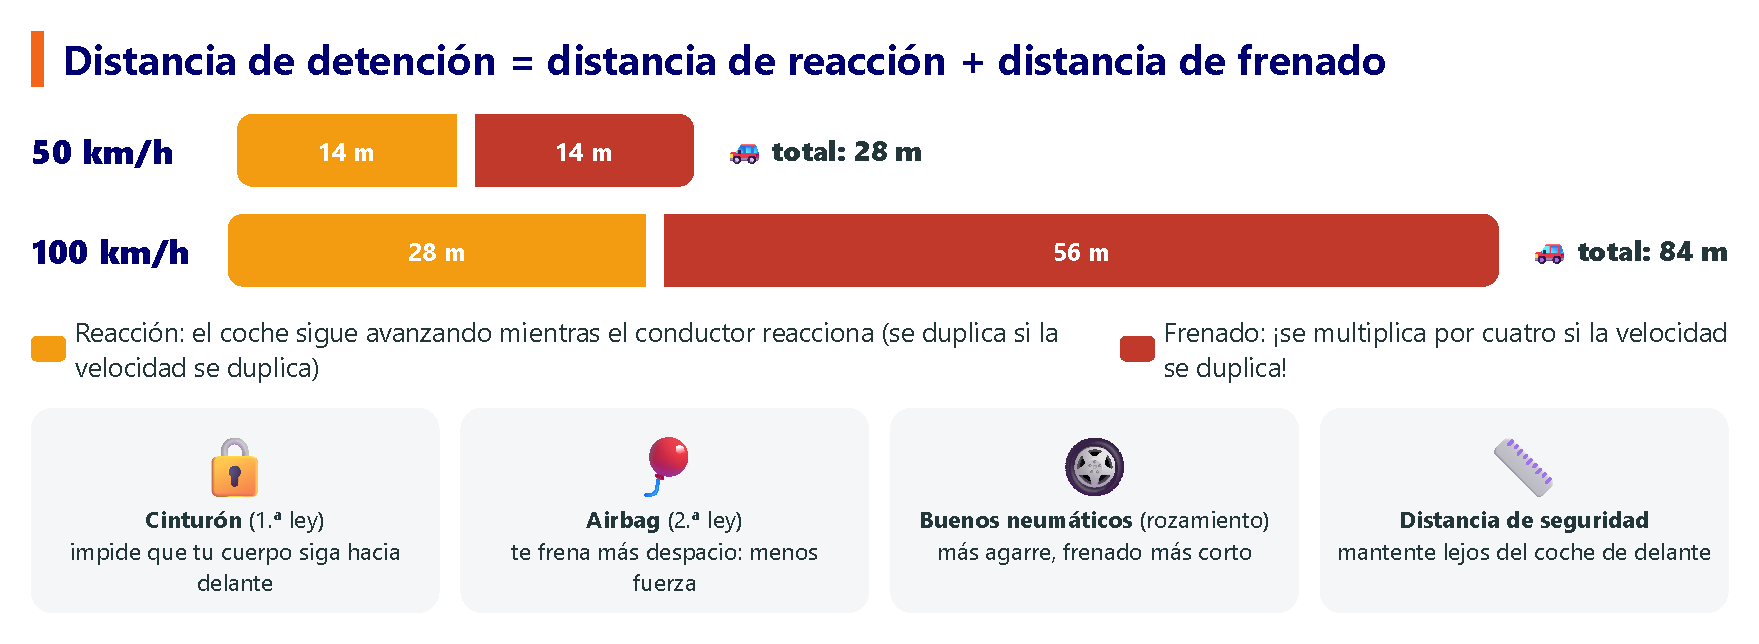
\includegraphics[width=\textwidth]{FigurasSVG/Unit_8_Forces/pdf/stopping_distance_es.pdf}
    \caption{Distancia de detención a dos velocidades (valores aproximados). Cuando la velocidad se duplica, la distancia de reacción se duplica, pero la distancia de frenado se multiplica por cuatro, así que la distancia total de detención se triplica.}
    \label{fig:u8_stopping_distance}
\end{figure}

\begin{didyouknow}
    Llevar puesto el cinturón de seguridad reduce más o menos a la mitad el riesgo de morir en un accidente de coche. En un choque a solo \qty{50}{\kmph}, un pasajero sin cinturón golpea el asiento de delante con una fuerza parecida al peso de un elefante.
\end{didyouknow}

\begin{exercise}
    Explica, con la primera ley de Newton (inercia), por qué los pasajeros de un coche deben llevar el cinturón de seguridad incluso en trayectos cortos y a poca velocidad.
    \begin{solu}
        Según la primera ley, el cuerpo de un pasajero en movimiento tiende a seguir moviéndose a la velocidad del coche mientras no actúe una fuerza sobre él. Si el coche choca y se para de golpe, sin cinturón el cuerpo del pasajero seguiría moviéndose hacia delante por inercia y podría golpearse contra el parabrisas o el asiento de delante. El cinturón aplica la fuerza necesaria para frenar al pasajero junto con el coche y evita que esto ocurra.
    \end{solu}
\end{exercise}

\begin{exercise}
    Un coche de \qty{1200}{\kg} de masa que frena en una carretera seca puede producir una fuerza de rozamiento (de frenado) máxima de \qty{6000}{\newton}.
    \begin{enumerate}[label=\letraminuscula]
        \item Calcula la deceleración máxima (en valor absoluto) que puede producir esta fuerza de frenado.
        \item Si la misma carretera está mojada y la fuerza de rozamiento máxima baja a \qty{3000}{\newton}, calcula la nueva deceleración máxima. Con la misma velocidad inicial, ¿la distancia de frenado es mayor o menor en la carretera mojada?
    \end{enumerate}
    \begin{solu}
        \begin{enumerate}[label=\alph*)]
            \item \(a = \dfrac{F}{m} = \dfrac{\qty{6000}{\newton}}{\qty{1200}{\kg}} = \qty{5}{\mpss}\).
            \item \(a = \dfrac{\qty{3000}{\newton}}{\qty{1200}{\kg}} = \qty{2.5}{\mpss}\). \\
            Como la deceleración es menor en la carretera mojada, el coche tarda \textbf{más tiempo y recorre más distancia} en pararse desde la misma velocidad: \textbf{la distancia de frenado es mayor}.
        \end{enumerate}
    \end{solu}
\end{exercise}

\begin{exercise}
    Una ciclista que va a \qty{10}{\mps} tarda \qty{0.5}{\s} en reaccionar antes de frenar (durante ese tiempo sigue moviéndose a velocidad constante). Cuando frena, decelera de manera uniforme a \qty{4}{\mpss} hasta pararse.
    \begin{enumerate}[label=\letraminuscula]
        \item Calcula la distancia que recorre durante el tiempo de reacción.
        \item Calcula cuánto tarda en pararse desde que empieza a frenar, y la distancia de frenado (con la fórmula del área del triángulo bajo la gráfica velocidad-tiempo).
        \item Calcula la distancia total de detención (distancia de reacción \(+\) distancia de frenado).
    \end{enumerate}
    \begin{solu}
        \begin{enumerate}[label=\alph*)]
            \item Distancia de reacción \(= v \cdot t_{\text{reacción}} = \qty{10}{\mps} \cdot \qty{0.5}{\s} = \qty{5}{\m}\).
            \item Tiempo para pararse: \(t = \dfrac{v_{\text{final}} - v_{\text{inicial}}}{a} = \dfrac{0 - \qty{10}{\mps}}{\qty{-4}{\mpss}} = \qty{2.5}{\s}\). \\
            Distancia de frenado \(= \dfrac{v_{\text{inicial}} \cdot t}{2} = \dfrac{\qty{10}{\mps} \cdot \qty{2.5}{\s}}{2} = \qty{12.5}{\m}\).
            \item Distancia total de detención \(= \qty{5}{\m} + \qty{12.5}{\m} = \qty{17.5}{\m}\): es la distancia de seguridad mínima que debe mantener con el vehículo de delante.
        \end{enumerate}
    \end{solu}
\end{exercise}

%----------------------------------------------------------------------------------------

\section{Fuerzas y deformación}

Cuando se aplica una fuerza que deforma, los objetos pueden comportarse de maneras distintas:

\begin{figure}[H]
    \centering
    % [FIGURA ORIGINAL] \includegraphics[width=\textwidth]{Unit_8/deformation}
    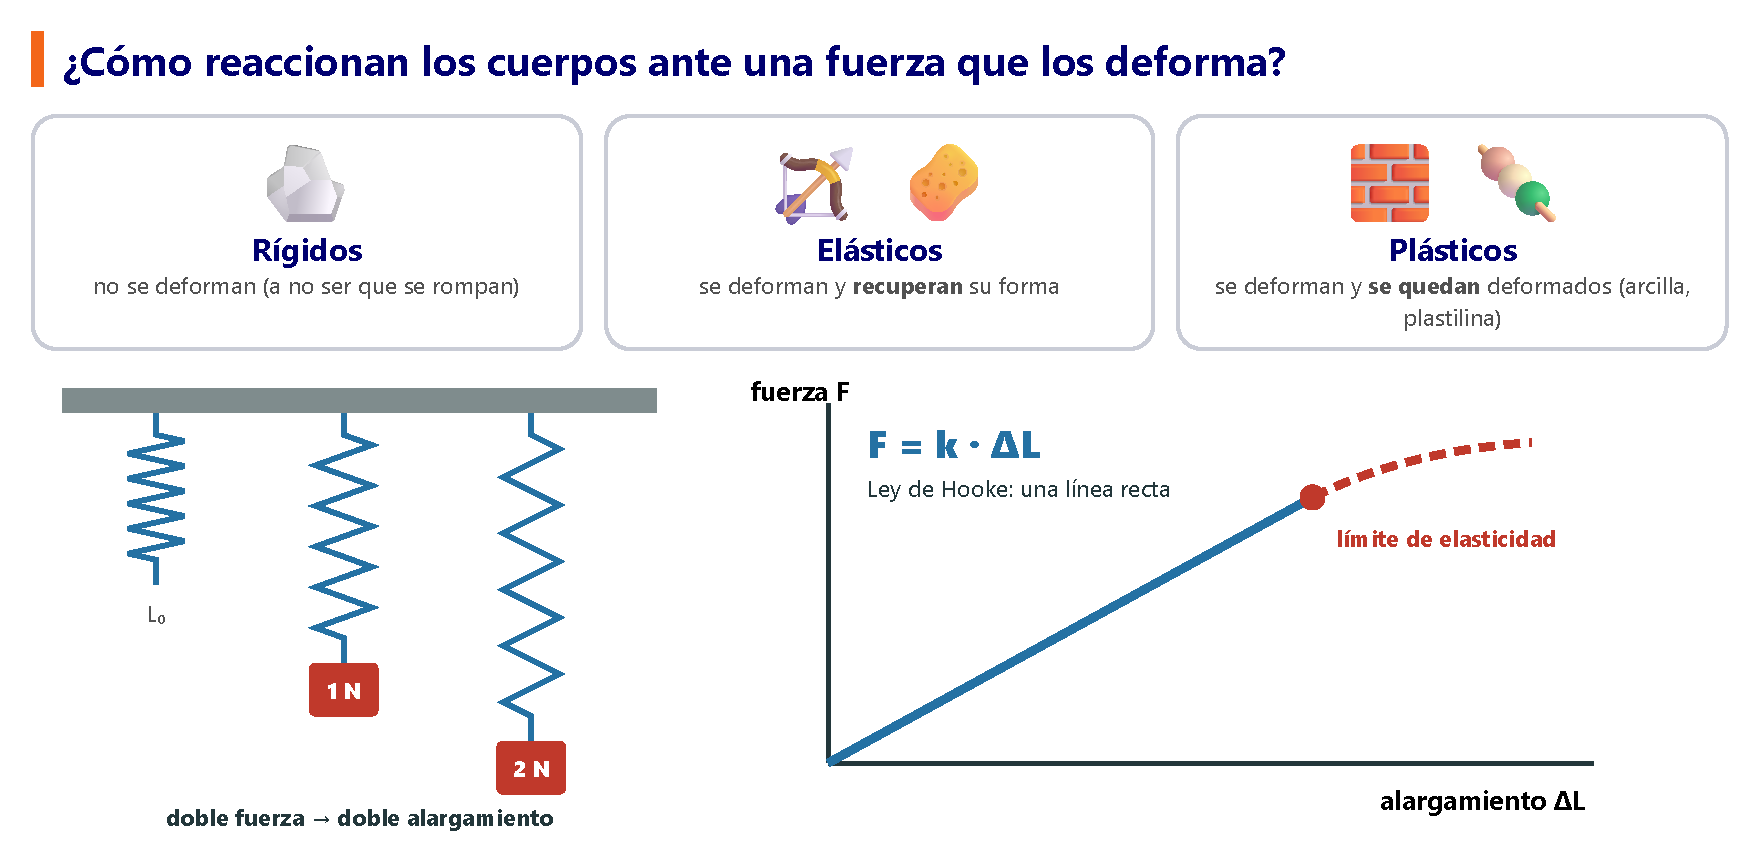
\includegraphics[width=\textwidth]{FigurasSVG/Unit_8_Forces/pdf/deformation_es.pdf}
    \caption{Cuerpos rígidos, elásticos y plásticos, y ley de Hooke para un muelle.}
    \label{fig:u8_deformation}
\end{figure}

\begin{impt}
    Una fuerza deformadora muy grande puede hacer que un cuerpo rígido supere su \negsubro{límite de rotura} y se rompa, o que un cuerpo elástico supere su \negsubro{límite de elasticidad} y se quede deformado para siempre.
\end{impt}

Las fuerzas se miden con un \negsubro{dinamómetro}: un muelle calibrado que se estira, o se comprime, en proporción a la fuerza aplicada.

\begin{definition}[Ley de Hooke]
    La deformación (alargamiento) de un muelle, \(\Delta L\), es directamente proporcional a la fuerza aplicada:
    \begin{equation*}
        F = k \cdot \Delta L
    \end{equation*}
    donde \(k\) es la \textbf{constante elástica}, una propiedad característica de cada muelle, que se mide en \unit{\newton\per\metre}.
\end{definition}

\begin{example}
    \textbf{Un muelle de \qty{20}{\cm} de longitud se estira hasta \qty{23}{\cm} cuando se tira de él con una fuerza de \qty{1.5}{\newton}. Calcula:}
    \begin{enumerate}[label=\letraminuscula]
        \item Su constante elástica.
        \item Su longitud cuando se tira de él con una fuerza de \qty{5}{\newton}.
    \end{enumerate}
    \begin{enumerate}[label=\alph*)]
        \item \(\Delta L = \qty{23}{\cm} - \qty{20}{\cm} = \qty{3}{\cm} = \qty{0.03}{\m}\). \\
        \(k = \dfrac{F}{\Delta L} = \dfrac{\qty{1.5}{\newton}}{\qty{0.03}{\m}} = \qty{50}{\newton\per\metre}\).
        \item \(\Delta L = \dfrac{F}{k} = \dfrac{\qty{5}{\newton}}{\qty{50}{\newton\per\metre}} = \qty{0.1}{\m} = \qty{10}{\cm}\). \\
        \(L = L_0 + \Delta L = \qty{20}{\cm} + \qty{10}{\cm} = \qty{30}{\cm}\).
    \end{enumerate}
\end{example}

\begin{exercise}
    Un muelle de \qty{20}{\cm} de longitud tiene una constante elástica de \qty{100}{\newton\per\metre}. Calcula la fuerza con la que hay que tirar de él para que se estire hasta \qty{23}{\cm}.
    \begin{solu}
        \(\Delta L = \qty{23}{\cm} - \qty{20}{\cm} = \qty{0.03}{\m}\). \\
        \(F = k \cdot \Delta L = \qty{100}{\newton\per\metre} \cdot \qty{0.03}{\m} = \qty{3}{\newton}\).
    \end{solu}
\end{exercise}

\begin{exercise}
    El muelle de una báscula de cocina mide \qty{5}{\cm} y tiene una constante elástica de \qty{800}{\newton\per\metre}. Se coloca sobre la báscula un objeto que pesa \qty{8}{\newton}.
    \begin{enumerate}[label=\letraminuscula]
        \item ¿Cuánto mide ahora el muelle?
    \end{enumerate}
    \begin{solu}
        \(\Delta L = \dfrac{F}{k} = \dfrac{\qty{8}{\newton}}{\qty{800}{\newton\per\metre}} = \qty{0.01}{\m} = \qty{1}{\cm}\). \\
        \(L = L_0 + \Delta L = \qty{5}{\cm} + \qty{1}{\cm} = \qty{6}{\cm}\).
    \end{solu}
\end{exercise}

\begin{exercise}
    Dos muelles, \(A\) y \(B\), se estiran con la misma fuerza de \qty{4}{\newton}. El muelle \(A\) se alarga \qty{2}{\cm} y el muelle \(B\) se alarga \qty{5}{\cm}.
    \begin{enumerate}[label=\letraminuscula]
        \item Calcula la constante elástica de cada muelle.
        \item ¿Qué muelle es más «duro» (cuesta más estirarlo)? Justifica tu respuesta con el valor de \(k\).
    \end{enumerate}
    \begin{solu}
        \begin{enumerate}[label=\alph*)]
            \item \(k_A = \dfrac{F}{\Delta L} = \dfrac{\qty{4}{\newton}}{\qty{0.02}{\m}} = \qty{200}{\newton\per\metre}\). \\
            \(k_B = \dfrac{F}{\Delta L} = \dfrac{\qty{4}{\newton}}{\qty{0.05}{\m}} = \qty{80}{\newton\per\metre}\).
            \item El muelle \(A\) es más duro, porque tiene una constante elástica \textbf{mayor}: con la misma fuerza se estira menos, así que hace falta más fuerza para producirle una misma deformación.
        \end{enumerate}
    \end{solu}
\end{exercise}

\begin{exercise}
    Un muelle tiene una longitud natural de \qty{15}{\cm}. Cuando se le aplica una fuerza de \qty{6}{\newton}, se estira hasta \qty{21}{\cm}.
    \begin{enumerate}[label=\letraminuscula]
        \item Calcula su constante elástica.
        \item El límite de elasticidad del muelle corresponde a un alargamiento máximo de \qty{10}{\cm}. ¿Cuál es la fuerza máxima que puede soportar sin dejar de comportarse como un cuerpo elástico?
    \end{enumerate}
    \begin{solu}
        \begin{enumerate}[label=\alph*)]
            \item \(\Delta L = \qty{21}{\cm} - \qty{15}{\cm} = \qty{6}{\cm} = \qty{0.06}{\m}\). \\
            \(k = \dfrac{F}{\Delta L} = \dfrac{\qty{6}{\newton}}{\qty{0.06}{\m}} = \qty{100}{\newton\per\metre}\).
            \item \(F_{\text{máx}} = k \cdot \Delta L_{\text{máx}} = \qty{100}{\newton\per\metre} \cdot \qty{0.10}{\m} = \qty{10}{\newton}\).
        \end{enumerate}
    \end{solu}
\end{exercise}

%----------------------------------------------------------------------------------------

%----------------------------------------------------------------------------------------

\section*{Resumen}

\begin{itemize}
    \item \textbf{Leyes de Newton}: 1.ª (inercia: sin fuerza neta \(\to\) el movimiento no cambia); 2.ª (\(F = m \cdot a\)); 3.ª (acción y reacción, sobre cuerpos distintos).
    \item \textbf{Peso y masa}: la masa (\(m\), kg) no cambia; el peso (\(P = m \cdot g\), N) es una fuerza y cambia con \(g\).
    \item El \textbf{rozamiento} se opone al movimiento entre dos superficies en contacto; es fundamental en la seguridad vial, junto con el cinturón, el airbag y unas distancias de frenado y de seguridad adecuadas (aplicaciones de las leyes de Newton).
    \item \textbf{Deformación}: rígidos (no se deforman), elásticos (recuperan su forma), plásticos (se quedan deformados). \textbf{Ley de Hooke}: \(F = k \cdot \Delta L\).
\end{itemize}

\section{Vocabulario}

\begin{vocabulary}[Inercia (\textit{inertia})]
    Tendencia de un objeto a mantener su estado de movimiento (reposo o MRU) mientras no actúe sobre él una fuerza neta.
\end{vocabulary}

\begin{vocabulary}[Fuerza neta o resultante (\textit{net force})]
    Fuerza total que actúa sobre un objeto; se obtiene sumando todas las fuerzas que actúan sobre él.
\end{vocabulary}

\begin{vocabulary}[Dinamómetro (\textit{dynamometer})]
    Instrumento que sirve para medir fuerzas; funciona con un muelle calibrado.
\end{vocabulary}

\begin{vocabulary}[Límite de elasticidad (\textit{elastic limit})]
    Deformación máxima que puede sufrir un cuerpo elástico y aun así recuperar su forma original.
\end{vocabulary}

\begin{vocabulary}[Peso (\textit{weight})]
    Fuerza con la que un astro atrae a una masa hacia su centro; \(P = m \cdot g\).
\end{vocabulary}

\begin{vocabulary}[Masa (\textit{mass})]
    Cantidad de materia de un cuerpo; no cambia de un lugar a otro.
\end{vocabulary}

\begin{vocabulary}[Fuerza de rozamiento (\textit{friction force})]
    Fuerza que se opone al movimiento entre dos superficies que están en contacto.
\end{vocabulary}

\begin{vocabulary}[Distancia de frenado (\textit{braking distance})]
    Distancia que recorre un vehículo desde que se pisa el freno hasta que se para.
\end{vocabulary}
